\chapter{Implementation}
\label{cha:implementation}
Chapter~\ref{cha:design} gives a rough overview of what the individual building blocks in our system are responsible for and how the system is structured as a whole. In this chapter, we take a closer look at the individual parts and how they are implemented to provide the necessary functionality. While we go into more detail about the implementation of our system, we also mention some of the challenges we encountered while developing our system and how we overcame them. 

~\\
In Section~\ref{sec:reverse_proxy} we introduce the reverse proxy, its forwarding mechanics, and the messages that update these endpoints. 
The orchestrator contains the tools to manage the caching layers. Section~\ref{sec:orchestrator} describes those tools and introduces the endpoint scheduler, which uses these tools in the form of an event-based reactive mechanism, and is thus responsible for decision-making and setting up the caching layer. The storage backend and caching layer are also briefly covered; since S3 (see Section~\ref{sec:storage_backend}) and Redis (see Section~\ref{sec:self_hosted_redis}) do not require implementation, the focus is on the Lambda runtime (see Section~\ref{sec:serverless}). We explain how we leverage the serverless platform to create a server-like function that serves requests while AWS Lambda blocks incoming TCP connections. 

~\\
We chose Go as the implementation language for our system (orchestrator, reverse proxy, and Lambda runtime). Go is often used for cloud-based or server-side applications due to its high performance and built-in concurrency. The Go package \code{Redeo}~\cite{noauthor_redeo_nodate-1} was used to create Redis protocol-compatible TCP servers/services similar to InfiniCache~\cite{wang_infinicache_2020}.

\section{Reverse Proxy}
\label{sec:reverse_proxy}
The reverse proxy is the entry point for clients to retrieve key-value pairs by providing an API. Depending on the forwarding rules set by the orchestrator, the reverse proxy interacts with either the storage backend or the in-memory caching layer in the form of the Lambda runtime or self-hosted Redis. For the purposes of this work, we assume that the client is outside the AWS infrastructure without worrying about the actual client.

~\\ 
First, the reverse proxy implementation details are described in terms of startup and initialization. Then, the overall forwarding mechanic of the reverse proxy for API requests and how our system updates the endpoints are explained in more detail. 

\subsection{Startup}
At startup, the reverse proxy establishes a persistent TCP connection with the orchestrator, which is later used for client/server communication, with the reverse proxy acting as the client. The corresponding address of the EC2 instance running the orchestrator is determined using the AWS SDK and the hard-coded instance ID. The reverse proxy also starts two servers at startup, one for the orchestrator and the other for communication with the Lambda runtime. This way, we can provide a bidirectional client/server communication between the reverse proxy and the orchestrator. In order for the orchestrator and later the Lambda runtime environment to connect to the corresponding reverse proxy server, the reverse proxy sends a \emph{ProxyHello} message to the orchestrator after the connection is successfully established, which contains the required information about both server endpoints. Last but also most important, the reverse proxy launches an API with a corresponding \code{get} endpoint through which the client can request key-value pairs. The API is implemented with the Gin Web Framework\footnote{Uses the Go package \code{HttpRouter}~\cite{schmidt_httprouter_2022} compared to the Go standard package \code{net/http} for a powerful HTTP request router for better performance according to their documentation.}~\cite{noauthor_gin_2022}.

\subsection{Forwarding}
\label{subsec:forwarding}
The API endpoint for \code{get} requests on our reverse proxy must distinguish whether the requests need to be forwarded to backend storage or whether in-memory caching is available. In this section, we first describe how this forwarding process is implemented in more detail. We then address the challenge of forwarding requests to dynamic endpoints that can shut down at any time, called in-flight handling. Finally, we briefly discuss the messages that the reverse proxy receives responsible for keeping the endpoints up to date; when and which building blocks trigger these messages is described in their respective sections.

~\\
The reverse proxy uses a mapping for each key that is overwritten when changes are received for routing. As we will see later, multiple goroutines could read and overwrite these entries, so a safe mapping for concurrent use from the Go package \code{sync.map} is used. Controlled by this mapping, either S3, the running Lambda runtime, or the self-hosted Redis instance is queried. Before the request is forwarded, a goroutine sends a message to the orchestrator containing the key, the endpoint to use, and a Unix timestamp.

~\\
So far, we have only mentioned that the request is forwarded. We describe the implementation details depending on the endpoint in this section. For the backend storage and the self-hosted Redis, the process is basically the same, while for the Lambda runtime, we have to consider that the connection is not a traditional client/server connection. Accessing the storage backend is relatively self-evident with the \code{aws-sdk-go} for the S3 service. The value is downloaded and copied into the response and returned to the client. The package go-redis~\cite{noauthor_redis_nodate-1} is used to query the self-hosted Redis instance. The client is initialized with an address and password before the request arrives and then used to forward the request by using the \code{get} operation for the client. Section~\ref{subsec:lambda} explains connection management for the Lambda runtime in more detail and why we are not able to get the appropriate response to a request as in traditional client/server scenarios. While sending the request using the Lambda runtime client is straightforward, we have to make some additional preparations to receive the response. In addition to the key, we also send a universally unique identifier (UUID) in our \code{get} request. A go channel is created through which the response is forwarded by the goroutine handling the response. We store the channel in a mapping and use the UUID as the key to associate the response with the corresponding request. The response contains the UUID of the request so that the response handler can find the correct channel to forward the response to. Once we receive the response on the channel, it can be sent back to the client.

\subsubsection{In-Flight Handling} 
To prevent the case where our reverse proxy forwards a request to the caching layer while the corresponding layer is simultaneously shut down, we use two Reader/Writer mutual exclusion locks (\code{sync.RWMutex}). One for the self-hosted Redis and one for the Lambda runtime. Each time a request is forwarded, the goroutine handling the request claims the corresponding Read lock and releases the lock after the request is resolved. As long as a request for one of the caching layers is in-flight, claiming the Write lock will block. Both caching layers send a message to the reverse proxy before they shut down, asking the reverse proxy to acknowledge the message. So before we acknowledge such a message, the reverse proxy claims the Write lock, which is blocked as long as a request is in-flight. As soon as we claim it, we can safely confirm the shutdown. Updating the mapping beforehand prevents new requests from being in-flight for the given endpoint, so the caching layer can be safely turned off.

\subsubsection{Updates} 
Later in Section~\ref{sec:orchestrator}, we will see how the orchestrator makes decisions about the caching layer and how the two layers are started and handled. For now, we will focus only on the messages received by the reverse proxy and the resulting actions. The orchestrator receives the following messages:
\begin{itemize}
    \item \emph{RedisStart}: Contains the address of the self-hosted Redis instance used to initialize a new Redis client.
    \item \emph{RedisUpdate}: Informs the reverse proxy about added or removed keys in the Redis instance. Adding sets the corresponding mapping entry to the Redis endpoint, while removing deletes the entry.
    \item \emph{RedisStop}: Claims the Write lock for Redis, removes the Redis client and sends an acknowledgment back.  
\end{itemize}
Similar to the orchestrator, the Lambda runtime also sends two messages to the reverse proxy:
\begin{itemize}
    \item \emph{LambdaStart}: Contains the key that is now served by the Lambda runtime and sets the corresponding mapping entry to the Lambda endpoint.
    \item \emph{LambdaBye}: The message contains the key of the Lambda runtime that is currently being shut down. Checks the mapping and deletes the entry if the current Lambda endpoint is included. Otherwise, no action is taken, indicating that a message from the orchestrator has already overwritten the entry. Unlike the Redis shutdown acknowledgment mechanism, the message handler starts a goroutine that claims the Lambda Write lock and sends a separate acknowledge message instead of a response. This is necessary because bidirectional client/server communication with the Lambda runtime is not possible due to the limitation of incoming connections.
\end{itemize}

\section{Orchestrator}
\label{sec:orchestrator}
% Object Manager
% Self-hosted Redis instance management.
% Lambda function invoke handling.
The reverse proxy is responsible for actually forwarding the client requests, while the orchestrator works in the background to ensure that the reverse proxy operates as intended and that the corresponding in-memory caching layer is managed as expected. 

~\\
First, we cover the startup and initialization of the orchestrator. We then present the tools and implementation details that the orchestrator needs to manage the in-memory caching layers in Section~\ref{subsec:orchestration_cachinglayer}. We cover how the orchestrator manages the EC2 lifecycle for the self-hosted Redis instance and how the serverless functions are invoked as an additional in-memory caching layer. Section~\ref{subsec:endpoint_scheduler} then explains the reactive design of our system by introducing the orchestrator's endpoint scheduler, which is responsible for managing the in-memory caching layers based on a state diagram. The endpoint scheduler is modeled as a reactive event-based mechanism that uses a feedback loop with the reverse proxy for events and keeps the endpoints on the reverse proxy up to date.

% Section~\ref{subsec:endpoint_scheduler} then explains reactive design of our system by covering the logic behind the orchestrator, which we call the endpoint scheduler. The state of the current implementation models our endpoint scheduler as a reactive, event-based mechanism where events are messages from the proxy that inform our orchestrator of the latest requests served. Choosing a simple and transparent mechanism as our endpoint scheduler helped get the system up and running quickly and provide insight into the capabilities of our system. 

\subsection{Startup}
The startup is similar to the reverse proxy by starting two servers, one for the communication with the Lambda runtime and the other for the reverse proxy. The server for the reverse proxy is required once the proxy is up and running. Recall that one of the first actions of the reverse proxy after establishing a connection to the orchestrator is to send a startup message containing the addresses of the two endpoint servers running on the reverse proxy. After receiving the message, the orchestrator also establishes a persistent TCP connection to the reverse proxy for client/server communication. This time the orchestrator acts as a client resulting in the bidirectional client/server communication channel. In addition, the orchestrator loads a system configuration file at startup, which is explained in more detail in Section~\ref{subsec:endpoint_scheduler}. It also initializes the \emph{RedisServerInstance} structure, which is used when interacting with the self-hosted Redis instance to keep track of the status of the EC2 instance running the Redis server, elaborated in more detail below.

\paragraph{Development API.} At startup, the orchestrator sets up a publicly available API that can be used to test and control the system. This is not used by the system but is worth mentioning because it was used extensively for testing before the system ran properly in its entirety. It contains endpoints for starting and shutting down the self-hosted Redis instance and interacting with it using standard Redis operations and the \code{ping} command. The API also includes endpoints to start and stop the Lambda runtime and an additional endpoint to log the current state of the reverse proxy forwarding rules on the console.  

\subsection{Orchestration of the Caching Layer}
\label{subsec:orchestration_cachinglayer}
This section covers the actions performed by the orchestrator to start, set up, and stop the caching layer components. This includes the required communication with other parts of the system. In the next section on the endpoint scheduler, we will see how these actions are actually applied in the running system. The role of the orchestrator for the self-hosted Redis part is much more extensive than simply invoking the serverless function that acts as Lambda runtime. Therefore, in this section, we only briefly cover the invocation process, while Section~\ref{sec:serverless} explains in more detail the design of our serverless function that acts as a caching layer component.

\subsubsection{Self-hosted Redis} 
As mentioned in Section~\ref{subsec:ec2}, our self-hosted Redis server runs on the EC2 compute platform as a daemon. As soon as the instance is up, the daemon starts, and the corresponding Redis server is available a short time later. The general role of the orchestrator is to start the instance as soon as the self-hosted Redis cache layer is requested and to shut it down if we decide otherwise. To track the status of the instance, the orchestrator maintains the \emph{RedisServerInstance} structure containing the instance ID, the address, and the status. At startup, the structure is initialized by querying the status of the EC2 instance using the AWS SDK for the EC2 service and the hard-coded instance ID. The address is set when the instance enters the running state and removed when stopped. We use two levels of abstraction in the implementation, where the first level is at the Redis level, and the underlying level is about the EC2 instance running the daemon. The Redis layer interacts with the EC2 instance layer to start and stop the instance as needed. This abstraction serves to separate the tasks of each layer clearly. The EC2 layer is responsible for managing the lifecycle transitions of the EC2 instance and informing the Redis layer of the transitions. While the Redis layer initiates these state transitions, it ensures that the actual Redis server daemon is up and running and notifies the reverse proxy about it. Due to the time required for the state transitions and the startup time of the daemon, we designed those two layers in a non-blocking manner by using goroutines and channels to notify each other.

~\\
Initially, the instance is in the stopped state, and when the orchestrator decides to start the Redis server, we initiate the startup at the Redis layer. A channel can be provided that is used as a signaling mechanism to notify the caller when the Redis server is ready. The Redis layer initiates the EC2 startup at the second layer and again uses a signaling channel to be notified when the instance enters the running state. We get the address of the running EC2 instance on this channel, which is used to create a new Redis client. Using the Redis client, we periodically \code{ping} the Redis server. When we get back a successful \code{pong}, we know that the Redis server is up and running and inform the reverse proxy with the \emph{RedisStart} message, which provides it with the required address to create a Redis client itself.

~\\
When the orchestrator requests to stop the Redis server, we query the list of current keys and inform the reverse proxy in the \emph{RedisUpdate} about the removed keys. Afterward, we send the message \emph{RedisStop} to the reverse proxy, which uses the acknowledgment mechanism described above for in-flight requests. So after we receive the acknowledgment, we can safely delete the Redis key-value pairs, remove the Redis client, and finally shut down the EC2 instance using the second layer. The caller can provide a channel to get notified as soon as the instance enters the stopped state.

~\\
In Section~\ref{subsec:ec2} we discussed that the instance is only billed when it is in the running state; this is important later for evaluating the cost of our system. When we ask the Redis server to start, the provided channel is notified when the instance enters the running state and starts accounting. For shutdown requests, billing ends when the function returns, while the channel is used to notify when the instance enters the stopped state, which means we can restart the instance.

\subsubsection{Lambda Runtime} 
Starting the Lambda runtime is simply a matter of invoking the Lambda function using the AWS SDK for the Lambda service. The function is called synchronously with the function name and a payload received from the handler code as function arguments. The payload includes the key of the key-value pair to be served by the Lambda runtime and a \emph{TICK} duration, the use of which is explained in Section~\ref{sec:serverless}. Also, the payload contains two addresses, one for the orchestrator server and the other for the reverse proxy server (which was received in the \emph{ProxyHello} message). Remember that this call blocks because of the synchronous requests. Once the Invoke returns, the Lambda runtime environment has either finished executing, crashed, or reached the timeout limit.

\subsection{Endpoint Scheduler}
\label{subsec:endpoint_scheduler}
% explain the general concept of the endpoint scheduler
% reactive, event-based mechanism
% events are
Our orchestrator now has all the tools to start and manage the in-memory caching layer. What is still missing is the reactive event-based mechanism, the endpoint scheduler. We mentioned the endpoint scheduler and the state diagram that models the endpoint used by the reverse proxy. The endpoint scheduler maintains a state for each object and follows the state diagram shown in Figure~\ref{fig:endpoint_scheduler}. Requests received by the reverse proxy are used as events that, together with the current state and additional parameters, trigger the transition within the state diagram and thus change the endpoint on the reverse proxy. 

~\\
First, we provide an overview of the state diagram and our endpoint scheduler and describe the system parameters used in the state diagram. We then explain in detail the implementation of our reactive event-based mechanism. Finally, we introduce the system configurator, which is used to derive the required system parameters for our system.

\begin{figure}[t]
    \begin{center}
        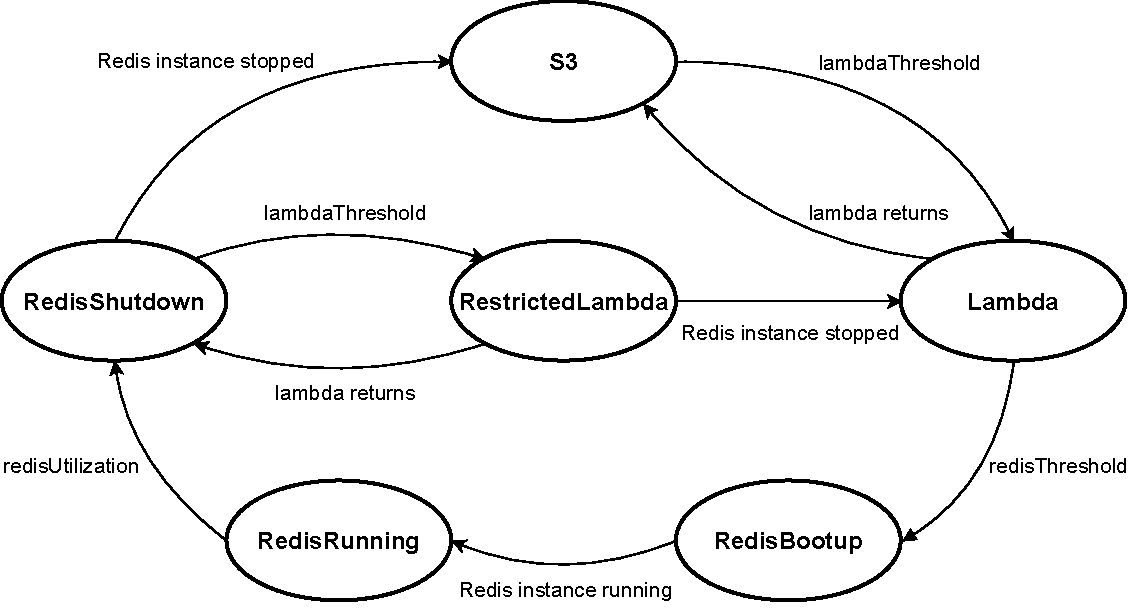
\includegraphics[width=0.8\textwidth]{figures/endpoint_scheduler.pdf}
        \caption{State diagram of the reactive, event-based endpoint scheduler.}
        \label{fig:endpoint_scheduler}
    \end{center}
\end{figure}

\subsubsection{State Diagram}
Initially, only the backend storage is available, which is referred to as state \textsc{S3}. We motivated serverless computing as a rapidly available additional in-memory caching layer. Thus, when our endpoint scheduler decides to provide in-memory caching, it switches to the \textsc{Lambda} state. This decision is based on a threshold for the number of requests received within a given time window. The following state transition is a bit more complicated due to the way we use the serverless platform, but simply put, the endpoint scheduler decides to either return to the \textsc{S3} state and turn off the serverless in-memory layer, or, if the load persists, use the less expensive self-hosted Redis layer. The time required to make the EC2 instance hosting Redis available is represented by the state \textsc{RedisBootup}. We continue to use the serverless platform for in-memory caching in this interim. Once the instance is up and running, the event-based design is suboptimal because we could get stuck in this state and the instance will be up and running forever. Therefore, to decide whether the endpoint scheduler should stop the Redis instance, a timer is used to re-evaluate the decision periodically. At this point, we cannot directly return to the \textsc{S3} state because the Redis instance is still shutting down, which prevents our system from restarting the instance immediately. To model this situation, we use the \textsc{RedisShutdown} state, which is basically the same as \textsc{S3}, except that when the serverless platform is restarted, the option to transition back to Redis is disabled until the instance is successfully stopped.

% The endpoint scheduler keeps a state for each key and follows a state diagram shown in Figure~\ref{fig:endpoint_scheduler}. The state transitions are based on thresholds and parameters defined in the system configuration, which is presented first. The diagram and the actions performed by the endpoint scheduler based on the state and events are then explained in more detail.

\subsubsection{System Parameters}
After a general introduction of the endpoint scheduler and the state diagram, we introduce the system parameters that play an essential role in the responsiveness and behavior of our endpoint scheduler since the transitions in the state diagram are directly coupled to them. Section~\ref{sec:endpoint_scheduler} in the evaluation examines their impact and their high dependence on the actual workload, while Section~\ref{subsec:system_configurator} shows how these parameters are derived. The parameters are loaded by the orchestrator from the local \code{conf.yaml} file at startup. To understand the next section about the implementation of the reactive event-based mechanism, we give a brief overview here:
\begin{itemize}
    \item \emph{TICK}: Used as argument for the Lambda runtime, and from then on serves as the \emph{TICK} duration for the timeout-based Lambda runtime described in Section~\ref{sec:serverless}.
    \item \emph{lambdaWindowElements}: Specifies the number of most recent requests to be considered when evaluating the \emph{lambdaThreshold}.
    \item \emph{lambdaThreshold}: Time duration, if the last requests defined by the \emph{lambdaWindowElements} value are within this duration, the threshold is exceeded.
    \item \emph{redisThreshold}: Specifies the number of requests that must be resolved from the current Lambda runtime to transition to the self-hosted Redis caching layer. 
    \item \emph{redisUtilization}: Time duration, shutdown of the Redis server if the last requests stored in the queue are not within this duration.
\end{itemize}
The state we keep for each key includes not only the state according to Figure~\ref{fig:endpoint_scheduler}, but also a counter called \emph{lambdaCount}, a queue that stores the timestamps of the last five requests, and a mutual exclusion lock which becomes more apparent when we explain the implementation of the reactive event-based mechanism in the next section.

\subsubsection{Reactive Event-Based Mechanism.}
It is important to note that anything that happens on the orchestrator does not directly affect the end-to-end latency of \code{get} requests. However, it is worth noting that the additional message that the reverse proxy sends to the orchestrator that forms the event for our event-based mechanism does impact end-to-end latency, but it is an asynchronous message sent via a goroutine, so it is not actually on the critical latency path but consumes CPU capacity on the reverse proxy. To reduce the number of messages sent by the reverse proxy to the orchestrator, the granularity of those messages could be reduced by transferring some logic to the reverse proxy and sending messages only after certain thresholds are exceeded. This would increase the reverse proxy work while reducing the number of messages transmitted. We chose to retain fine-grained messaging to avoid passing logic to the reverse proxy and to clearly separate forwarding and endpoint scheduling. The number of messages could be reduced, if necessary, by batch processing on the part of the reverse proxy, which would affect the responsiveness of our mechanism. Although the endpoint scheduler does not directly influence the end-to-end request latency, it is nevertheless closely linked. The result of our endpoint scheduler determines whether an in-memory caching layer is set up, which is directly reflected in the end-to-end latency of incoming requests by using the available caching layer.

~\\
The endpoint scheduler processes each event in the form of a message from the reverse proxy about a received request individually. The message contains the requested key and the timestamp when the reverse proxy received the request. When processing the event, the corresponding state of the specified key is retrieved first, and the mutex in the state is used to synchronize event processing for the same key. The timestamp is pushed back to the queue, and then the actual processing starts based on the current state. Figure~\ref{fig:endpoint_scheduler} provides an overview of all possible states. We try to keep the synchronized part of the processing as minimalistic as possible and use goroutines for more time-consuming tasks, carefully using the corresponding key's mutex to prevent concurrent state changes or interactions.

~\\
\textbf{\textsc{S3.}} We use the queue to calculate the time difference between the last timestamp and the timestamp specified by \emph{lambdaWindowElements}. The size of the queue limits the possible values for the \emph{lambdaWindowElements}, and we first check if enough timestamps have already been added to the queue. Suppose the calculated time difference is less than the duration of \emph{lambdaThreshold}. In that case, we enter the \textsc{Lambda} state and start a goroutine responsible for starting the Lambda runtime and handling the event when the function returns. When the function returns, the goroutine locks the mutex, resets the \emph{lambdaCount} to zero, and switches back to the \textsc{S3} state if we are still in the \textsc{Lambda} state.

~\\
\textbf{\textsc{Lambda.}} The Lambda runtime is either already running or is just being started in this state. So first, we increase the \emph{lambdaCount} and check the current value. If the value exceeds the \emph{redisThreshold}, we send the \emph{KeepRunning} message to the Lambda runtime and enter the \textsc{RedisBootup} state.\\
A goroutine is actually used to start the self-hosted Redis instance. Remember that we can provide a channel that will be notified when the Redis server is up and running and the Redis client is ready to use. Once the channel is notified, the goroutine proceeds to prepare the Redis server to serve the appropriate key by downloading the key-value pair from S3 and setting it up on the Redis server. We then send a \emph{RedisUpdate} message to the reverse proxy, which changes the forwarding to use the Redis server. While this whole process takes some time, we do not keep the mutex in the goroutine that is started after we transition to the \textsc{RedisBootup} state. But as soon as we have sent the message to the reverse proxy, we lock the mutex, transition into the \textsc{RedisRunning} state, and send the \emph{ManualShutdown} message to the Lambda runtime.\\
Finally, another goroutine manages how long the Redis server actually runs. While the event-based design works great for the Lambda runtime, which uses a timeout functionality, we need to use something similar for our Redis server because if no more events arrive, we would be stuck in the \textsc{RedisRunning} state. To solve this problem, the goroutine uses a \code{time.Ticker} with a period of one minute to periodically check if the Redis server should be stopped. The check first locks the mutex, and if the time difference between the last timestamp and the first timestamp in our queue is greater than the \emph{redisUtilization} duration, we stop the Redis server; otherwise, we check again later. After stopping the Redis server and transitioning to the \textsc{RedisShutdown} state, a goroutine waits on the notification channel signaling that the EC2 instance has transitioned to the stopped state. At this point, we lock the mutex and change the state depending on the current state. We are either in the \textsc{RedisShutdown} state and transition to the \textsc{S3} state, or we are in the \textsc{RestrictedLambda} state where we transition to the \textsc{Lambda} state. 
% shorten the lambda part

~\\
\textbf{\textsc{RedisBootup.}} In this state, there is no event-based action; the Lambda runtime is currently running with timeout disabled due to the \emph{KeepRunning} message. In the meantime, the Redis server is started and prepared to serve requests for the given key, which will lead to the transition to the next state as described above.

~\\
\textbf{\textsc{RedisRunning.}} Once we have transitioned to the \textsc{RedisRunning} state, the reverse proxy has been updated, and the Redis server from now on will serve requests for the key. No event-based actions are performed, but the periodic task explained above decides when to shut down the instance based on the timestamps in our queue and the \emph{redisUtilization}.

~\\
\textbf{\textsc{RedisShutdown.}} The process is similar to the \textsc{S3} state except that we change to the \textsc{RestrictedLambda} state compared to the \textsc{Lambda} state. The goroutine that handles the event when the function returns slightly differs depending on our state when the function returns. So if we are in the \textsc{Lambda} state, we move to the \textsc{S3} state, but if we are in the \textsc{RestrictedLambda} state, we move back to the \textsc{RedisShutdown} state.

~\\
\textbf{\textsc{RestrictedLambda.}} This state is similar to the \textsc{Lambda} state, which indicates a running Lambda runtime. However, compared to the \textsc{Lambda} state, we cannot currently start the Redis server because we are still in the process of shutting it down. Nevertheless, we increase the \emph{lambdaCount}, because as soon as the EC2 instance enters the stopped state, a state transition is triggered that depends on the current state, as described in the \textsc{Lambda} state. So if we are currently in the \textsc{RestrictedLambda} state, we will transition to the \textsc{Lambda} state, which indicates that we are now ready to restart the Redis server.

\subsection{System Configurator}
\label{subsec:system_configurator}
% show how we derive these parameters
% explain the initial thoughts for the sensitivity and rate input
With a better understanding of our reactive event-based mechanism, we now explain in more detail how we derive the system configuration parameters mentioned above. The tight dependence between the behavior or responsiveness of our endpoint scheduler and the workload distribution makes it difficult to design the system to perform well for every possible workload. To address this problem, we separate the system configuration parameters from the orchestrator to allow the user some flexibility in providing appropriate parameters at startup. The system parameters determine how quickly our system responds to backend storage accesses by starting a Lambda runtime, the granularity for the transition to the Redis layer, and the forgiveness with which each caching layer is kept operational with respect to the actual workload hitting our system. Choosing the appropriate parameters seems to be a hyperparameter optimization problem. However, without knowing the characteristics of the workload in advance, it is challenging to derive parameters that work well for each workload. We also work with a two-dimensional optimization problem, where we want to achieve the best performance (in-memory cache) while minimizing the cost of our system (minimize in-memory cache runtime). 

\newpage
\noindent
We try to solve this problem by providing a system configurator that runs on the EC2 instance of the orchestrator before we start the actual orchestrator. It receives some input from the system administrator and derives the system configuration parameters stored in the \code{conf.yaml} file. The input includes the expected rate of requests per object during a one-minute time interval and a sensitivity value, which should reflect how important it is for the system administrator to have in-memory caching. The rate is needed to get a general understanding of the expected time between requests, while the sensitivity is used to define the forgiveness mentioned above. Thus, a higher sensitivity value leads to longer availability of in-memory caching but also higher costs. The system configurator is designed as a step function, a linear combination of the rate and the sensitivity value. We originally thought this was crucial, but Section~\ref{sec:endpoint_scheduler} in the evaluation will show some limitations of our system for general workloads, while it becomes less important for peak workloads as shown in Section~\ref{subsec:peak_workload}. The explicit calculations of the system configurator can be found in the Appendix~\ref{sec:system_configurator_algorithm}. 

\section{Storage Backend}
\label{sec:storage_backend}
S3 forms the persistent storage backend part of our system for the key-value pairs. If no in-memory caching is required, the client interacts directly with the storage backend without a reverse proxy in between. Our system, specifically the reverse proxy, uses the S3 API to retrieve key-value pairs when in-memory caching is not available for client requests. The other parts of our system also use the storage backend when setting up the in-memory caching layer. In the case of self-hosted Redis, the orchestrator is responsible for retrieving the key-value pairs and setting them up on the Redis instance. In contrast, the Lambda runtime queries the storage backend itself for the key specified in the Invoke arguments.

\section{Serverless}
\label{sec:serverless}
We leverage the AWS Lambda serverless platform by using a function as an in-memory caching component. Our function is designed to act as a server in the client/server design principle, allowing our reverse proxy to forward \code{get} requests to the Lambda runtime, which previously fetched the object from the storage backend at startup. The orchestrator invokes the Lambda runtime and communicates with the reverse proxy when it can be used as the endpoint of the caching layer. The lifetime of the function is managed by a timeout that is extended when requests are received. The maximum lifetime is limited by the concept of transitioning to the self-hosted Redis caching layer when demand persists. Otherwise, the timeout function forces the Lambda runtime to shut down.

\subsection{Startup}
% Lambda Communication explanation.
% Object retrieval.
Section~\ref{subsec:lambda} covers all the background of how AWS Lambda starts a function, up to the point where the actual function code is executed. The initialization code covers everything before we start the handler code, where we get the payload mentioned in Section~\ref{subsec:orchestration_cachinglayer} as function arguments: the key, the \emph{TICK}, and two endpoint addresses. Our initialization code creates two servers and registers the specific handler functions for the servers. As mentioned in Section~\ref{subsec:lambda}, reuse of the execution environments will result in state still being available to our function, so most of the operations now described are designed in the manner of get or create to take advantage of the case where the function is invoked as a warm startup.

\newpage
\noindent
The handler code starts by setting up the runtime, which is responsible for managing the timeout of our function. The initial timeout duration is set accordingly to the \emph{TICK} argument and continuously checked using a goroutine. The key argument represents the key-value pair that the Lambda runtime should cache. If the mapping is empty, we download the key-value pair from S3 and update the corresponding mapping. This way, in the case of a warm startup, we do not download an existing value. Then, we establish the connection to the endpoints specified in the arguments and start serving the created servers through these connections. One connection is intended for communication with the orchestrator, the other for reverse proxy communication. At this point, we send the \emph{LambdaStart} message to the reverse proxy, which contains the keys provided by the Lambda runtime that overrides the forwarding rule if the backend storage previously provided the key. The Lambda runtime acts as a server for requests from the reverse proxy and commands from the orchestrator.

\subsection{Runtime}
% Runtime management and timer functionality (extending, in-flight handling).
The function continues execution until either the timeout expires or we receive the \emph{ManualShutdown} message from the orchestrator. The lambda runtime is waiting on two channels, with each channel used to notify the occurrence of one of the above events. If such an event occurs, we send the \emph{LambdaBye} message to the reverse proxy and block until we receive the acknowledgment as described in Section~\ref{subsec:forwarding}. With this mechanism, the Lambda runtime environment continues to serve requests sent before the reverse proxy was notified of the shutdown but prevents new requests from being forwarded to the Lambda runtime. After the acknowledgment is received, the Lambda runtime returns, at which point the synchronous function Invoke by the orchestrator returns.

~\\
The timeout duration was initially set to the \emph{TICK} duration. However, our runtime managing the timeout functionality extends this timeout by an additional \emph{TICK} for each \code{get} request we receive from the reverse proxy. Once we receive the \emph{KeepRunning} message from the orchestrator indicating that we are about to start the self-hosted Redis server, we disable the timeout extension feature for \code{get} requests. We do not entirely disable the timeout to avoid implementation issues where the function continues to run until the function-specific timeout of four minutes is reached (we set this timeout to four minutes to avoid unnecessary billing time during development). Instead, when we receive the \emph{KeepRunning} message, we extend the timeout by two minutes and disable the feature to extend it as described above. In this way, the function will run until we receive the \emph{ManualShutdown} message indicating that the self-hosted Redis server is running, and the Lambda runtime is no longer needed.

\subsection{Connection Management}
We repeatedly mentioned the lack of bidirectional client/server communication when the Lambda runtime was involved. We briefly covered the issue of AWS Lambda functions not allowing incoming TCP or UDP connections in Section~\ref{subsec:lambda}. This section describes how we overcome this issue to achieve bidirectional communication. As described in the startup section, two servers are started, one for the orchestrator and the other for the reverse proxy. For a traditional server, we specify a listener for the server to serve on, which then accepts incoming connections on the listener and serves each client. A handler function should be registered for each command that the server offers.

\newpage
\noindent
However, this is impossible for the Lambda runtime because no incoming connections are allowed. So, unlike the traditional server setup with a listener, the Lambda runtime connects to the specified endpoints provided at startup and serves the previously established connection based on the mentioned \code{Redeo} package, similar to how InfiniCache~\cite{wang_infinicache_2020} solves this problem. The way to register handler functions for the Lambda runtime server is the same as for traditional servers. 

~\\
The other part of the connection (orchestrator or reverse proxy) sets up a server with a listener at startup itself, which is precisely the endpoint provided to the Lambda runtime as invoke argument. So when the Lambda runtime establishes the connection, the counterpart accepts the incoming connection and creates a new client with the associated connection, through which requests can be sent to the Lambda runtime. At the same time, we have a goroutine that handles all incoming requests on the connection from the Lambda runtime. In this way, we can provide bidirectional client/server communication between the Lambda runtime and its counterpart with only one connection established by the Lambda runtime. The drawback of this approach is that the complexity of mapping a response to a request is shifted to the application layer since we cannot distinguish between requests and responses as described in Section~\ref{subsec:forwarding}.

\section{Self-Hosted Redis}
\label{sec:self_hosted_redis}
Self-hosted Redis on EC2 is used as an in-memory caching component similar to the serverless platform. The reverse proxy can forward requests by querying the Redis instance directly. Unlike the Lambda runtime, the orchestrator is responsible for managing the entire lifecycle of the Redis instance, so only the orchestrator tells the reverse proxy if Redis is available, which keys are being served, and when the keys are no longer available because the instance is shut down. We decided to use the Redis instance as a start-and-forget caching layer by removing the keys when the instance is shut down. Therefore, the orchestrator is responsible for setting up the keys to be served by the Redis instance by downloading them from the backend store and issuing Redis commands. We avoid using Redis features to maintain the database after a restart, such as writing snapshots to disk or keeping an append-only file used to replay operations on restart. This avoids unpredictable startup times for our Redis instance due to the extra time required to set up the correct database state and avoids inconsistent data in the caching layer.